\begin{abstract}
Paired spectra can distinguish a shared absorption feature from additional attenuation only when wavelength registration and intensity normalization are preserved. The data contain twenty-one wavelength bins from 400 to 700~nm, with sample, star-only, continuum-reference and dark intensities. At 595~nm the sample is 55.2\% below the entered continuum reference, but the star-only spectrum already contains a substantial depression. Dividing the two dark-subtracted spectra leaves an additional depth of 0.132, only 0.0225 above the neighbouring-bin baseline. The 15-nm sampling interval describes broad spectral sampling; narrow-line identification also depends on the instrumental line-spread function. The analysis relates these distinctions to transmission spectroscopy and shows why wavelength calibration uncertainty alone cannot establish spectral resolution or detection significance.
\end{abstract}
\begin{IEEEkeywords}
Spectral ratios, transmission spectroscopy, wavelength calibration, resolving power, continuum normalization.
\end{IEEEkeywords}

\section{A spectral feature needs a comparison}
The physical meaning of a dark interval depends on the spectrum used as its reference. A stellar absorption line, a terrestrial absorber, a filter and a reduction artifact can all lower the detected intensity. Transit spectroscopy therefore compares spectra obtained in different configurations while retaining the stellar contribution. Seager and Sasselov developed predictions for atmospheric signatures superimposed on stellar radiation\cite{seager2000}; Brown formulated wavelength-dependent spectrum ratios and examined their dependence on atmospheric structure\cite{brown2001}. The classroom comparison considered here retains that logic while treating the extra absorber as a separate sample.

A useful scale comparison is the sodium result of Charbonneau et al.\cite{charbonneau2002}: their differential transit depth was $(2.32\pm0.57)\times10^{-4}$ in a specifically defined bandpass. The additional depths in the present example are of order $10^{-1}$. They illustrate normalization and shared-feature rejection, rather than the observing precision or geometric dilution of an actual exoplanet atmosphere. Passing all source light through a filter does not reproduce the small atmospheric annulus of a transiting planet.

Each detected bin is itself an optical integral. For configuration $i$ and bin $j$, a linear model is
\begin{equation}
 C_{ij}=D_j+g_it_i\int L_j(\lambda)\eta(\lambda)F_i(\lambda)\,d\lambda,
 \label{eq:spectral-fingerprints-response}
\end{equation}
where $L_j$ describes the bin and instrumental line-spread function, $\eta$ the spectral response, and $D_j$ the dark offset. A ratio of these integrals is generally a weighted mean, not the monochromatic transmission at the labelled centre. This distinction becomes decisive when the bins are wider than the feature of interest.

\section{Matched wavelength and intensity scales}
A separate wavelength-calibrated spectrometer supplies the intensities. The comparison is transferred manually; three broad RGB channels cannot supply resolved line measurements. Figure~\ref{fig:spectral-fingerprints-apparatus} shows an interchangeable sample in a fixed optical path. Source-only, sample, continuum-reference and covered-detector observations must share slit geometry, detector response, exposure and gain, or be corrected to a common linear intensity scale. Independent peak normalization would remove some real attenuation and change the additional-depth estimator.

\begin{figure}[t]
\centering
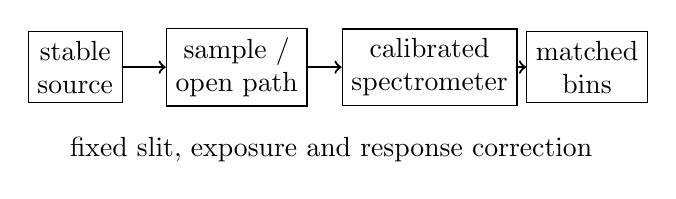
\begin{tikzpicture}[x=1cm,y=1cm]
 \node[draw,align=center] (source) at (0.65,0.8) {stable\\source};
 \node[draw,align=center] (holder) at (2.7,0.8) {sample /\\open path};
 \node[draw,align=center] (spec) at (5.15,0.8) {calibrated\\spectrometer};
 \node[draw,align=center] (roi) at (7.15,0.8) {matched\\bins};
 \draw[->,thick] (source)--(holder);\draw[->,thick] (holder)--(spec);
 \draw[->,thick] (spec)--(roi);
 \node[align=center] at (3.9,-0.25) {fixed slit, exposure and response correction};
\end{tikzpicture}
\caption{Apparatus schematic. A separate spectrometer observes matched optical configurations. A covered-detector observation supplies the dark correction; all comparisons retain a common wavelength grid.}
\label{fig:spectral-fingerprints-apparatus}
\end{figure}

Let $S,A,R,D$ denote sample, star-only, continuum-reference and dark intensity at one common wavelength. The normalized spectra and additional depth are
\begin{align}
 T_S&=\frac{S-D}{R-D},&T_A&=\frac{A-D}{R-D},\\
 d_{\rm add}&=1-\frac{T_S}{T_A}
            =1-\frac{S-D}{A-D}.
 \label{eq:spectral-fingerprints-ratio}
\end{align}
The shared continuum reference cancels algebraically from $d_{\rm add}$. It remains essential to the separate normalized spectra and to defining an apparent line depth $1-T_S$. A near-zero star-only denominator amplifies noise, so no additional depth should be assigned there. Saturation invalidates the assumed linear ratios even if a subsequent normalization gives an innocuous value.

The example uses a common dark intensity of 2 arbitrary units, a ceiling of 200 and twenty-one checked wavelength pairs. All listed signals lie below that ceiling. Every result is evaluated at its actual calibrated wavelength, in 15-nm increments; the observation index is not used as a spectral coordinate. A separately entered comparison wavelength is a candidate location, not an identification assigned by the analysis.

\begin{figure}[t]
\centering
% Generated by prepare_drafts.py from the supplied CSV files.
\begin{tikzpicture}
\begin{groupplot}[group style={group size=1 by 2,vertical sep=1.15cm},
width=0.98\columnwidth,height=3.4cm,
grid=major,enlarge x limits=false,
legend style={font=\scriptsize,at={(0.5,1.03)},anchor=south,
legend columns=4,draw=none,fill=none,column sep=4pt},
title style={font=\scriptsize,at={(0.02,0.98)},anchor=north west,
fill=white,fill opacity=0.9,text opacity=1,inner sep=2pt},
ylabel style={font=\footnotesize},
xlabel style={font=\footnotesize},tick label style={font=\scriptsize}]
\nextgroupplot[ylabel={Normalized intensity}]
\addplot[csblue,solid,line width=0.8pt,mark=*] table[col sep=comma,x=c1,y expr={(\thisrow{c10}-(0))*(1)}] {data/drafts/spectral-fingerprints.csv};
\addlegendentry{Sample}
\addplot[csred,dashed,line width=0.8pt,mark=square*] table[col sep=comma,x=c1,y expr={(\thisrow{c11}-(0))*(1)}] {data/drafts/spectral-fingerprints.csv};
\addlegendentry{Star-only}
\nextgroupplot[ylabel={Additional depth},xlabel={Wavelength (nm)}]
\addplot[csteal,dashdotted,line width=0.8pt,mark=*] table[col sep=comma,x=c1,y expr={(\thisrow{c13}-(0))*(1)}] {data/drafts/spectral-fingerprints.csv};
\end{groupplot}
\end{tikzpicture}

\caption{Upper: dark-subtracted sample and star-only intensities divided by the common continuum reference. Lower: additional depth $1-(S-D)/(A-D)$. Points are spaced by 15~nm; connecting lines guide the eye.}
\label{fig:spectral-fingerprints-data}
\end{figure}

\section{A shared depression near 595~nm}
The most pronounced sample depression occurs at 595~nm, where $T_S=0.4479$ and $T_A=0.5162$. Relative to the entered continuum reference, the apparent sample depth is 0.5521. Much of this depression is shared by the star-only comparison. The additional depth after division is 0.1323, as Table~\ref{tab:spectral-fingerprints-results} shows.

\begin{table}[t]
\caption{Normalized sample and star-only signals and additional attenuation depth at four wavelengths.}
\label{tab:spectral-fingerprints-results}
\centering\footnotesize
\begin{tabular}{@{}rrrr@{}}
\toprule
$\lambda$ (nm)&$T_S$&$T_A$&$d_{\rm add}$\\
\midrule
580&0.6260&0.7031&0.1097\\
595&0.4479&0.5162&0.1323\\
610&0.6348&0.7131&0.1097\\
655&0.6019&0.7103&0.1526\\
\bottomrule
\end{tabular}
\end{table}

For an explicit local comparison, take the arithmetic mean of the 580- and 610-nm bins as a straight-line continuum at 595~nm. The resulting local depressions are 28.94\% for the sample and 27.10\% for the star-only spectrum. Applying the same neighbouring-bin baseline to $d_{\rm add}$ leaves an excess of 0.0225, or 2.25 percentage points. This is a descriptive local contrast, not a fitted line equivalent width. A curved continuum or a broad overlapping band would change it.

Across 400--700~nm, additional depth ranges from 0.1097 to 0.2973. This broad variation remains after the shared feature is suppressed. The 55.2\% depression relative to the continuum reference therefore cannot be assigned entirely to the extra absorber. Shared features and broad attenuation must be separated before interpreting a local residual. The data instead support broad selective attenuation plus a modest local departure near a shared depression.

\section{Resolution and identifiability}
The entered wavelength uncertainty is 0.2~nm, whereas the grid spacing is 15~nm. These quantities describe different properties. Calibration uncertainty concerns the wavelength assigned to a bin; resolution depends on the instrumental line-spread function and the available sampling. Robertson shows why even a line-spread function's FWHM does not define a universal resolving-power comparison\cite{robertson2013}. The ratio $\lambda/(15\unit{nm})$ describes the sampling scale; measured resolving power additionally depends on the instrumental width.

The sodium D components tabulated by NIST lie near 589.0 and 589.6~nm\cite{nistasd2024}. Their approximately 0.5974-nm separation is about twenty-five times smaller than the example grid interval. The 595-nm point is also 6~nm from the entered 589-nm comparison value. Species assignment uses the resolved profile, several consistent features, the instrumental response and the treatment of stellar and terrestrial contributions.

The 0.0225 local excess is the measured additional-depth contrast. Its detection significance depends on the intensity uncertainties and covariance of the paired spectra. Uncertainty in a shared dark estimate correlates wavelength ratios, and imperfect wavelength registration can leave a false differential feature where a stellar spectrum has a steep slope. These effects must enter a covariance model or repeated matched observations before interpreting a residual chemically. The present comparison establishes how normalization changes the physical question; it does not uniquely determine composition, temperature or atmospheric abundance.
